%%%%%%%%%%%%%%%%%%%%%%%%%%%%%%
% 統計学の知識のインデックス(「統計学図鑑」)
%%%%%%%%%%%%%%%%%%%%%%%%%%%%%%

\part{統計学インデックス}

統計学図鑑\cite{統計学図鑑}を参考に,統計学のインデックスを作成する.
統計学の基礎部分の体系がどのようになっているかをざっと確認できるようにするのが目的.

%%%%%%%%%%%%%%%%%%%%%%%%%%%%%%
% chapter 統計学とは
%%%%%%%%%%%%%%%%%%%%%%%%%%%%%%

\chapter{統計学とは}

\section{統計学の分類}

統計学の分類を確認する.

\begin{itemize}
  \item 統計学・・・対象集団,現象の特徴を把握する方法を体系化した学問
        \begin{itemize}
          \item 記述統計学・・・手元のデータの特徴を捉える(平均,ばらつき,相関係数など)
          \item 推測統計学・・・手元のデータの特徴を捉える(点推定,区間推定,仮説検定)
                \begin{itemize}
                  \item 頻度論的統計学・・・一般的な統計学
                  \item ベイズ統計学(ベイズ統計学を推測統計学に含めないとする考え方もある)
                \end{itemize}
        \end{itemize}
\end{itemize}

%%%%%%%%%%%%%%%%%%%%%%%%%%%%%%
% chapter 記述統計学
%%%%%%%%%%%%%%%%%%%%%%%%%%%%%%

\chapter{記述統計学}

% section: 代表値
\section{代表値}
\subsection{平均値}
\subsection{中央値}
\subsection{最頻値}

\section{データのばらつき}
\subsection{分散,標準偏差}
\subsection{分位数}
\subsection{変動係数}

「相対標準偏差」と言われれば一発で理解できる.

\begin{itemize}
  \item 変動係数 coefficient of variattion,CV
        \begin{itemize}
          \item 標準偏差を相対化した数値.標準偏差を平均値で割ったもの.「\textbf{相対標準偏差}」ともいう.
          \item 各群の標準偏差を平均値で補正することで,\textbf{単位,平均値が異なる群間のばらつきを比較することができる.}
        \end{itemize}
\end{itemize}

\begin{align}
  CV = \frac{\sqrt{s}}{\bar{x}}
\end{align}

% section: 変量の関連性
\section{変量の関連性}

\subsection{相関係数}

\subsubsection{ピアソンの積率相関係数}

一般に,「相関係数」と言った場合「ピアソンの積率相関係数」を指すことが多い.

\subsection{順位相関係数}

\begin{itemize}
  \item 順位相関係数
        \begin{itemize}
          \item 2 つの順序変数間の相関の強さを測る指標.
                「スピアマンの順位相関係数」と「ケンドーコバヤシの順位相関係数」がある.どちらの指標を用いるかに明確な基準はない(要出典).
        \end{itemize}
\end{itemize}

\subsubsection{スピアマンの順位相関係数}

順位データに対して「ピアソンの積率相関係数」を計算した数値が「\textbf{スピアマンの積率相関係数}」である.
データが連続的な値を取る場合,まず順位データに変換する.

\subsubsection{ケンドールの順位相関係数}

%%%%%%%%%%%%%%%%%%%%%%%%%%%%%%
% chapter 確率分布
%%%%%%%%%%%%%%%%%%%%%%%%%%%%%%

\chapter{確率分布}

\section{確率変数,確率分布}

%%%%%%%%%%%%%%%%%%%%%%%%%%%%%%
% chapter 誤差論
%%%%%%%%%%%%%%%%%%%%%%%%%%%%%%

\chapter{誤差論}

\section{有効数字}
\section{系統誤差と偶然誤差}
\section{誤差の伝搬}

全ての計算を終えてから計算を行うか,間に平均などの集計を挟んで計算を行うか.
後者の場合,誤差の扱いが難しい.

%%%%%%%%%%%%%%%%%%%%%%%%%%%%%%
% chapter 推定
%%%%%%%%%%%%%%%%%%%%%%%%%%%%%%

\chapter{推定}

\section{何を「推定」するのか:母数}

推定の対象は,母数と呼ばれる母集団分布の特徴を表す定数である.

\begin{itemize}
  \item 母数 parameter
        \begin{itemize}
          \item 母集団分布の特徴を表す定数.
          \item 母平均,母分散,母標準偏差など.
        \end{itemize}
\end{itemize}



\section{統計量}
\section{統計的推測における「正規分布を仮定する」という前提}

流れの中で,今どんな前提条件,または仮定の元で論理を進めているか意識する必要がある.

\section{点推定}

母数を「1 点の数値」として推定する.
幅を持たない推定.

\subsection{推定量}
\subsection{最尤推定}
\subsection{モーメントを用いた推定}
\subsection{推定量の満たすべき性質}

\section{区間推定}

母数を「取りうる値の区間」として推定.
幅を持たせた推定.

\subsection{標本分布}

統計量が従う確率分布のこと.

\subsection{母平均の信頼区間}
\subsection{母比率の信頼区間}
\subsection{母分散の信頼区間}
\subsection{母相関係数の信頼区間}
\subsection{母相関係数の信頼区間}

\subsection{シミュレーションで母数を推定する:ブートストラップ法}
\subsubsection{ブートストラップ法}

\begin{itemize}
  \item ブートストラップ法
        \begin{itemize}
          \item 手元にある n 個のデータから同じサイズの再標本を何度も復元抽出し,その再標本の統計量から母数を推定する統計手法.
          \item 手元のデータから復元抽出を繰り返して(リサンプリング)たくさんの再標本を生成し,その統計量から母数を推定する方法.
          \item 小標本の場合など,母集団に確率分布が仮定できなくても母数の推定を可能にする.
          \item 統計学における「モンテカルロ法(コンピュータ・シミュレーション法)」の 1 つだが,乱数を用いず,実際にあるデータを使って分布を推定する.
        \end{itemize}
\end{itemize}

手元にある少ないデータだけで母数を高い精度で推定するにはどうすればいいか考えた時,

\subsubsection{母集団分布に正規性を過程できない}

区間推定では母集団分布が正規性であることを仮定することが多いが,
正規性を無理に仮定して t 分布を用いて推定しても,誤差が多すぎて実用に絶えない推定になる(信頼区間が広すぎるなど).

%%%%%%%%%%%%%%%%%%%%%%%%%%%%%%
% chapter 仮説検定
%%%%%%%%%%%%%%%%%%%%%%%%%%%%%%

\chapter{仮説検定}

\section{仮説検定とは}

帰無分布・・・帰無仮説が正しいものとして考えた時の標本分布.

\section{仮説検定の分類:パラメトリック検定とノンパラメトリック検定}
\section{帰無仮説と対立仮説}
\section{仮説検定の手順}

どのタイミングで「母集団分布」を仮定するのかに注意する.

\newpage

\section{仮説検定におけるリスク:第一種の過誤,第二種の過誤}

\subsection{第一種の過誤,第二種の過誤を図表で理解する}

どっちがどっちかややこしいけど,以下の画像を見ればすっきりする.

\begin{figure}[H]
  \begin{center}
    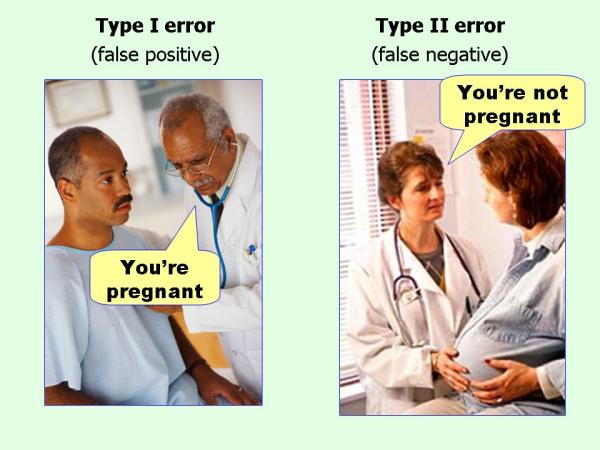
\includegraphics[width=15cm]{images/parts/4/type-i-and-type-ii-errors.jpg}
    \caption{第一種の過誤(偽陽性),第二種の過誤(偽陰性)}
  \end{center}
\end{figure}

(引用元:\linedhref{https://effectsizefaq.com/2010/05/31/i-always-get-confused-about-type-i-and-ii-errors-can-you-show-me-something-to-help-me-remember-the-difference/}{I always get confused about Type I and II errors. Can you show me something to help me remember the difference?})\\

ただ,上記画像だけでは理解が不十分.
第一種の過誤,第二種の過誤を犯してしまう際,それぞれを犯す確率というのが算出できる.
それを確率分布の図で表したものが以下.

\begin{figure}[H]
  \begin{center}
    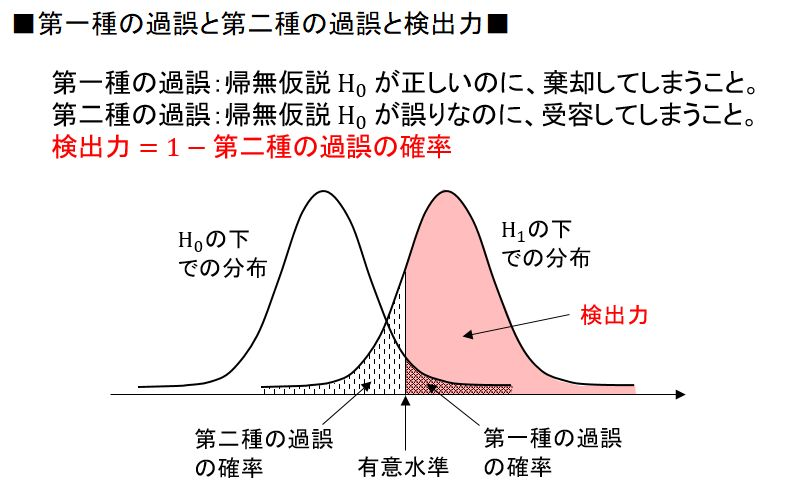
\includegraphics[width=15cm]{images/parts/4/pd-type-i-and-type-ii-errors.jpeg}
    \caption{確率分布で見る第一種の過誤(偽陽性),第二種の過誤(偽陰性)}
  \end{center}
\end{figure}

(引用元:\linedhref{https://twitter.com/ERUin2525/status/1168527197285445632}{Twitter より})\\

よく見る,第一種の過誤,第二種の過誤を整理した表は以下.
この表だけに頼ると永遠に忘れ続ける.ただし,下記画像の「差があると判断」は正しくない.
帰無仮説を「差が無い」としたとき,帰無仮説を棄却した結果主張できるのは「差が無いとは言えない」である(結果的に「差がある」と判断するだけれど)である.

(この主張↑間違っている可能性あり.「判断」だから間違いでは無い?)

\begin{figure}[H]
  \begin{center}
    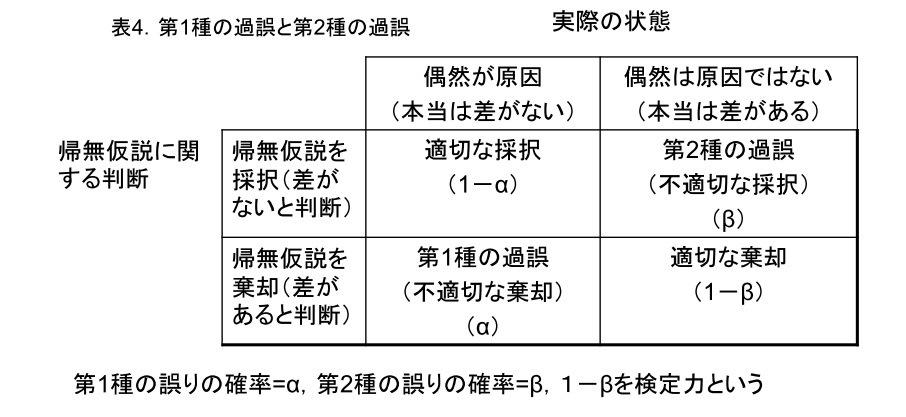
\includegraphics[width=15cm]{images/parts/4/table-type-i-and-type-ii-errors.jpeg}
    \caption{表で見る第一種の過誤(偽陽性),第二種の過誤(偽陰性)}
  \end{center}
\end{figure}

(引用元:\linedhref{https://twitter.com/kokushigou/status/529220780534411264}{Twitter より})\\

\newpage

\subsection{「第一種の過誤=有意水準」の意味するところ}

ここまでで,なぜ「第一種の過誤=有意水準(危険率)」なのかと疑問に思った.それに対する回答を以下に述べる.\\

有意水準は,「帰無分布に従うある事象が起こる確率が,有意水準より低かったら確率的に起こりにくいことであるとみなす(帰無分布から取り出される確率が低いとみなす)」という意味の(人為的な)基準である.
しかし,ある事象が起こる確率が有意水準より低くても,実は「その事象が(起こる確率は低くとも)帰無分布から発生した事象である」ということがありうる.

つまり,実際には帰無仮説が正しいのに,(人為的に決めた)棄却域に入っている値を帰無分布からサンプリングしてしまったが故に,
仮説検定によって有意だと検出されてしまったということである.

有意水準 $\alpha = 0.05$ のとき,\textbf{帰無分布からサンプリングすると $0.05$ の確率で棄却域に存在する標本を抽出してしまう}.
そして,この棄却域から抽出した標本に対して仮説検定を行うと有意だと判定されてしまう.
「実際には違うのに,有意だと判定されてしまう」,つまり,これが「偽陽性」であり,
サンプリングしたときに第一種の過誤が起こる確率が有意水準である $0.05$ そのものなのである.
「有意水準」は,第一種の過誤を起こしてしまう\emph{危険}性を数値的に示す値として「\textbf{危険率}」とも呼ばれる.

\section{母比率の検定}
\section{母分散の検定}
\section{相関の有無の判定:無相関の検定}

ただし,相関係数は「線形な」相関関係を示すものであり,「非線形な」関係の相関は表現できない.

\section{平均値の差の検定:対応のない 2 群の検定}

ほとんどの生物実験.

\section{平均値の差の検定:対応のある 2 群の検定}

マウスの血圧測定.

\section{比率の差の検定:対応のない 2 群の場合}
\section{非劣性試験}

%%%%%%%%%%%%%%%%%%%%%%%%%%%%%%
% chapter 分散分析
%%%%%%%%%%%%%%%%%%%%%%%%%%%%%%

\chapter{分散分析}

ANOVA(ANalysis Of VAriance)

\section{一元配置分散分析:実験で効果を確かめる}
\section{多群の等分散の検定:Bartlett 検定}
\section{対応のある一元配置分散分析:個体差を考慮する}
\section{二元配置分散分析:交互作用を見つけ出す}

%%%%%%%%%%%%%%%%%%%%%%%%%%%%%%
% chapter 検定の多重性
%%%%%%%%%%%%%%%%%%%%%%%%%%%%%%

\chapter{検定の多重性}

\section{検定の多重性とは}
\section{多重検定補正}
\subsection{Bonferrorni 法}

かなり厳しい多重検定補正の手法.

\subsection{Benjamini-Hochberg 法}

\linedhref{https://stats.biopapyrus.jp/stats/fdr-bh.html}{Benjamini-Hochberg 法:FDR を制御して多重比較検定補正を行う方法}

\section{Storey 法}
\section{Tukey 法,Tukey-Kramer 法}
\section{Dunnett 法}

%%%%%%%%%%%%%%%%%%%%%%%%%%%%%%
% chapter ノンパラメトリック検定
%%%%%%%%%%%%%%%%%%%%%%%%%%%%%%

\chapter{ノンパラメトリック検定}

\section{ノンパラメトリック検定:分布によらない仮説検定}

\begin{itemize}
  \item パラメトリック検定・・・母集団分布を仮定した仮説検定.
  \item ノンパラメトリック検定・・・母集団分布を仮定しない仮説検定.
\end{itemize}

\section{独立性の検定(ピアソンの $\chi^{2}$ 検定):質的データの検定}

\section{フィッシャーの正確確率検定:2 $\times$ 2 分割表の検定}
\section{対応のない 2 群の順序データの検定:マンホイットニーの U 検定}
\section{対応のある 2 群の順序データの検定:符号検定}
\section{対応のある 2 群の量的データの検定:ウィルコクソンの符号付き順位和検定}
\section{対応のない多群の順序データの検定:クラスカル・ウォリス検定}
\section{対応のある多群の順序データの検定:フリードマン検定}

%%%%%%%%%%%%%%%%%%%%%%%%%%%%%%
% chapter 実験計画法
%%%%%%%%%%%%%%%%%%%%%%%%%%%%%%

\chapter{実験計画法}

\section{フィッシャーの 3 原則:1 反復}
\section{フィッシャーの 3 原則:2 無作為化}
\section{フィッシャーの 3 原則:3 局所管理}
\section{色々な実験配置}
\section{直交計画法:実験を間引いて実施する}
\section{直交計画法の応用 1:品質工学(パラメータ設計)}
\section{直交計画法の応用 2:コンジョイント分析}

\section{検出力分析:標本サイズの決め方}
\subsection{検出力とは}
\subsection{検出力分析}

\subsection{補足:サンプルサイズとサンプル数}

\begin{itemize}
  \item サンプルサイズ,標本サイズ,sample size
        \begin{itemize}
          \item 1 標本に含まれる観測データの個数.
        \end{itemize}
  \item サンプル数,標本数,the number of samples
        \begin{itemize}
          \item 抽出した標本の数.つまり,何回標本抽出したかを表す数.
        \end{itemize}
\end{itemize}

%%%%%%%%%%%%%%%%%%%%%%%%%%%%%%
% chapter 回帰分析
%%%%%%%%%%%%%%%%%%%%%%%%%%%%%%

\chapter{回帰分析}

\section{回帰分析:原因と結果の関係を探る}
\section{最小二乗法}
\section{決定係数:回帰線の精度を評価する}
\section{t 検定:回帰線の傾きを検定する}
\section{残差分析:分析の適切さを検討する}

\section{重回帰分析:原因が複数あるときの回帰分析}
\subsection{多重共線性:説明変数間の問題}

略して「マルチコ」と呼ばれることもある.

\section{変数選択法:有効な説明変数を選ぶ}
\section{質の違いを説明する変数 1:切片ダミー}
\section{質の違いを説明する変数 2:傾きダミー}
\section{プロビット分析:2 値変数の回帰分析}
\section{イベント発生までの時間を分析する 1:生存曲線}
\section{イベント発生までの時間を分析する 2:生存曲線の比較}
\section{イベント発生までの時間を分析する 3:Cox 比例ハザード回帰}

%%%%%%%%%%%%%%%%%%%%%%%%%%%%%%
% chapter 多変量解析
%%%%%%%%%%%%%%%%%%%%%%%%%%%%%%

\chapter{多変量解析}

\section{多変量とは}

多変量データの意味から言えば,「単回帰分析」,「重回帰分析」も多変量解析に入るが,
前章で扱ったためこの章では扱わない.

\section{主成分分析:情報を縮約する}

次元削減,次元圧縮

\section{因子分析:潜在的な要因を発見する}
\section{多次元尺度構成法 MDS}
\section{クラスタリング}

神嶌先生のリンクが非常に分かりやすい.

\begin{itemize}
  \item クラスタリングの参考リンク
        \begin{itemize}
          \item \linedhref{http://www.kamishima.net/jp/kaisetsu/}{神嶌 敏弘:クラスタリング Clustering}
          \item \linedhref{http://www.kamishima.net/jp/clustering/}{クラスタリング(クラスター分析)}
        \end{itemize}
\end{itemize}

\subsection{非階層的クラスタリング}

\begin{itemize}
  \item kmeans 法
\end{itemize}

\subsection{階層的クラスタリング}

\begin{itemize}
  \item 最短距離法 nearest neighbor method
  \item 最長距離法 furthest neighbor method(完全連結法 complete linkage method)
  \item 群平均法 group average method
  \item ウォード法 Ward's method
\end{itemize}

\subsection{重要:クラスタリングの結果の解釈}

最も重要な点は,クラスタリングは探索的(exploratory)なデータ解析手法であり,クラスタリングによる分割は分析者のなんらかの主観や視点に基づいている,ということである.
よって,クラスタリングした結果は,データの要約などの知見を得るために用い,客観的な証拠として用いてはならない.

\section{構造方程式モデリング(SEM):因果構造を記述する}
\section{コレスポンデンス分析:質的データの関連性を分析する}
\section{数量化 1 類}
\section{数量化 2 類}
\section{数量化 3 類}

%%%%%%%%%%%%%%%%%%%%%%%%%%%%%%
% chapter 統計モデリング
%%%%%%%%%%%%%%%%%%%%%%%%%%%%%%

\chapter{統計モデリング}

\section{統計モデルとは}
\section{統計モデルの種類と発展}

\begin{figure}[H]
  \begin{center}
    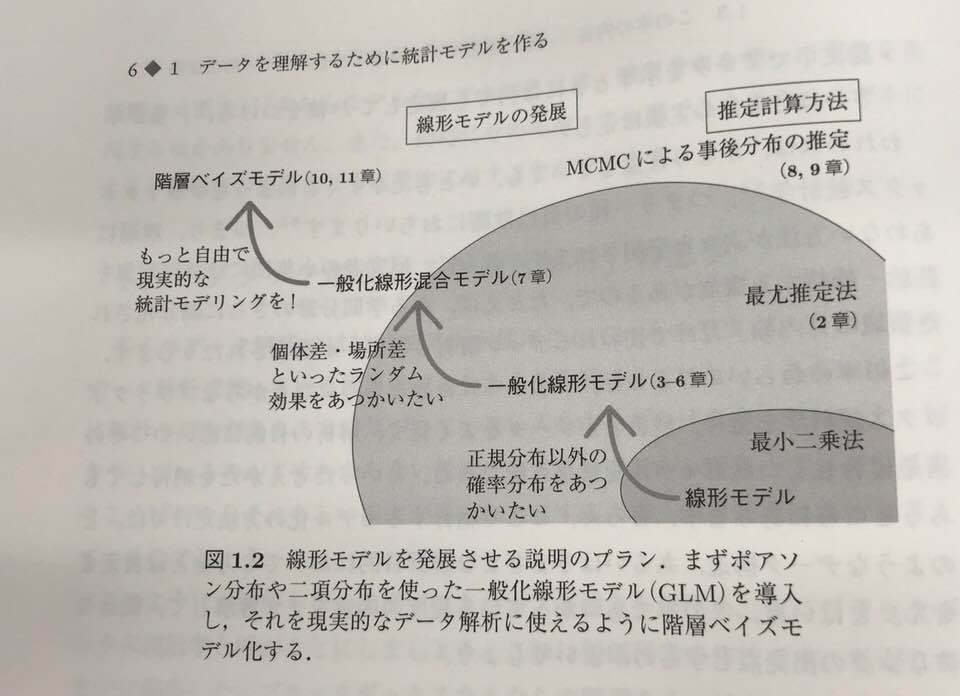
\includegraphics[width=15cm]{images/parts/4/statistical-model.jpg}
    \caption{統計モデルの発展}
  \end{center}
\end{figure}

\section{線形モデル}
\subsection{最小二乗法}

\section{一般化線形モデル}
\subsection{最尤推定法によるパラメータ推定}

\section{一般化線形混合モデル}
\section{階層ベイズモデル}

%%%%%%%%%%%%%%%%%%%%%%%%%%%%%%
% chapter 統計的因果推論
%%%%%%%%%%%%%%%%%%%%%%%%%%%%%%

\chapter{統計的因果推論}

%%%%%%%%%%%%%%%%%%%%%%%%%%%%%%
% chapter ベイズ統計学:基本
%%%%%%%%%%%%%%%%%%%%%%%%%%%%%%

\chapter{ベイズ統計学:基本}